\chapter{Tema 1: Introducción al machine learning}

\section{Métodos de partición de datos}

Al usar aprendizaje automático, los datos se pueden dividir de muchas
formas en entrenamiento y test. Algunas de las más comunes son:

\begin{enumerate}
    \item \textbf{Resustitución:}
    \begin{itemize}
        \item Todos los datos para entrenar y validar.
        \item Inconveniente: es muy optimista, ya que el modelo se ajusta
        a los datos con los los que se testea.
    \end{itemize}
    \item \textbf{Partición:}
    \begin{itemize}
        \item Se crea un subconjunto de datos para entrenar y otro para
        testear.
        \item Se puede hacer partición aleatoria o estratificada.
        \item Inconveniente: se desaprovechan datos.
    \end{itemize}
    \item \textbf{Validación cruzada en k bloques} (k-fold cross-validation):
    \begin{itemize}
        \item Se divide en k bloques y se entrena con k-1 bloques y se
        testea con el restante.
        \item Se repite k veces.
        \item Se promedian los resultados.
        \item Inconveniente: es costoso computacionalmente y se entrena
        con menos datos.
    \end{itemize}
    \item \textbf{Exclusión individual} (Leaving-one-out):
    \begin{itemize}
        \item Cada dato individual se usa para testear un sistema entrenado
        con el resto (n-1) de individuos.
        \item Equivale a k-fold con k=n.
        \item Inconveniente: es muy costoso computacionalmente.
    \end{itemize}
\end{enumerate}

\subsection{Métodos de partición gráficamente}

\begin{figure}[H]
    \centering
    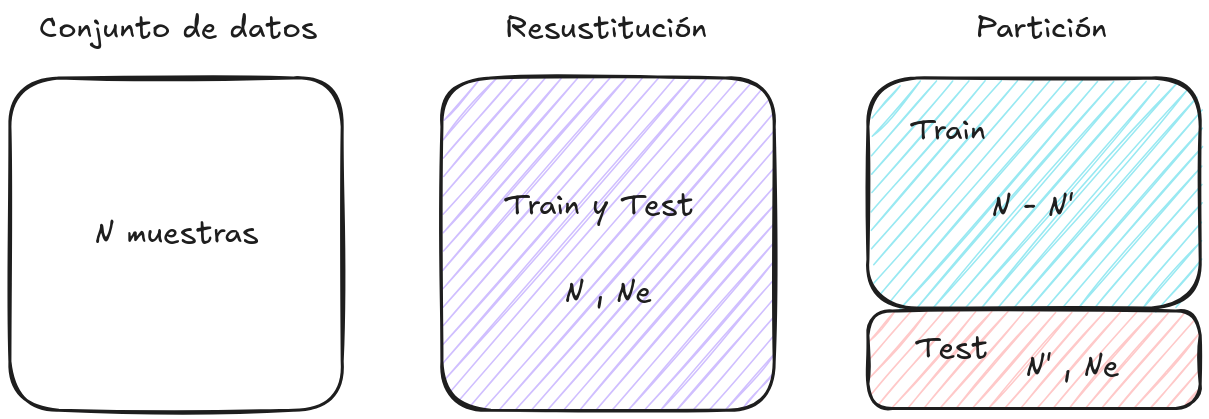
\includegraphics[width=0.8\textwidth]{images/particion.png}
    \caption{Partición de datos por resustitución y partición}
    \label{fig:particion_datos}
\end{figure}

En las imágenes, $N$ es el número de datos, $N_e$ es el número de errores,
$N'$ es el número de datos de testeo y $N'_e$ es el número de errores en test.

Para el método de partición, la tasa de errores se calcula como $\frac{N_e}{N}$
y la talla de entrenamiento efectiva es $N$.

En el método de partición, la tasa de errores se calcula como $\frac{N'_e}{N'}$
y la talla de entrenamiento efectiva es $N - N'$.

\begin{figure}[H]
    \centering
    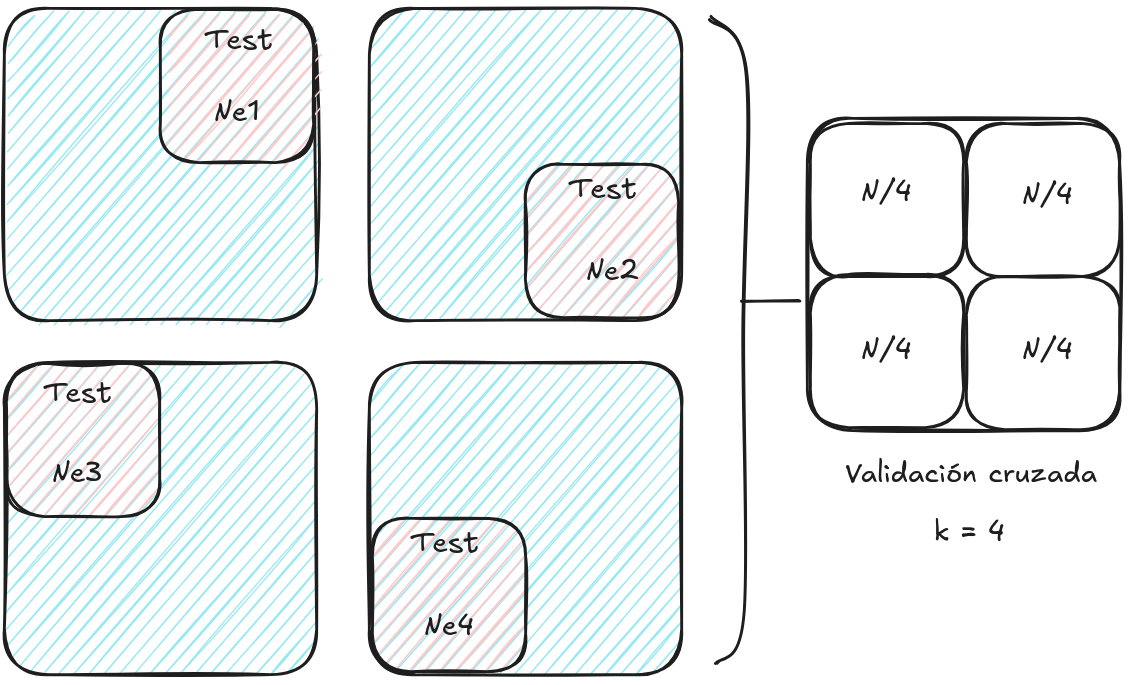
\includegraphics[width=0.8\textwidth]{images/cross_val.png}
    \caption{Validación cruzada con k = 4}
    \label{fig:cross_validation}
\end{figure}

Para la validación cruzada, la tasa de errores se calcula como
$\frac{N_{e1} + N_{e2} + N_{e3} + N_{e4}}{N}$ y la talla de entrenamiento
efectiva es $\frac{3N}{4}$.

De forma general, la tasa de errores se calcula como
$\frac{1}{k} \sum_{i=1}^{k} N_{ei}$ y la talla de entrenamiento efectiva es
$\frac{k-1}{k} N$.